\documentclass[12pt, a4paper, tocpage=plain]{abnt} % Fonte tamanho 12, papel A4, páginas do sumário sem o p.<número da página>

\usepackage[utf8]{inputenc} % dá suporte para caracteres especiais como acentos e cedilha
\usepackage[brazil]{babel} % Gera datas e nomes em português com estilo brasileiro
\usepackage{hyperref} % permite a criação de hyperlink no documento, como os links usados na referência
\usepackage[alf]{abntcite} % estilo de referência bibliográfica
\usepackage{graphicx} % Permite a utilização de imagens no documento
\usepackage[small]{caption} %Define as legendas das figuras com fontes menores do que o texto
\usepackage{pslatex} % Define que o formatao da letra será Times New Roman
\usepackage{epigraph} % Permite a criação de epígrafes 
\usepackage{setspace} % Permite a definição de espaçamento entre linhas
\usepackage[top=3cm, left=3cm, right=2cm, bottom=2cm]{geometry} % define as margens da folha

\setcounter{secnumdepth}{3} % Subsubsections numeradas
\setcounter{tocdepth}{3} % Subsubsections numeradas

\setlength{\parindent}{1.25cm} % Definição do recuo da primeira linha dos parágrafos para 1.25 cm

\renewcommand{\ABNTchapterfont}{\bfseries} %Define a fonte do \chapter
\renewcommand{\ABNTchaptersize}{\large} % Define o tamanho da fonte do \chapter
\renewcommand{\ABNTsectionfontsize}{\large} % Define o tamanho da fonte da \section
\renewcommand{\ABNTsubsectionfontsize}{\large} % Define o tamanho da fonte do \subsection
\renewcommand{\ABNTsubsubsectionfontsize}{\large} % Define o tamanho da fonte do \subsubsection
\renewcommand{\ABNTbibliographyname}{REFERÊNCIAS BIBLIOGRÁFICAS} % muda o título gerado pelo \bibliographys
\renewcommand{\ABNTanapsize}{\large} % Define o tamanho da fonte do \apendice
\renewcommand{\ABNTaposindicativoanap}{\centering} % Centraliza o título do apêndice

%\setlength{\parskip}{0pt}
%\setlength{\parsep}{0pt}
%\setlength{\headsep}{0pt}
%\setlength{\topskip}{0pt}
%\setlength{\topmargin}{0pt}
%\setlength{\topsep}{0pt}
%\setlength{\partopsep}{0pt}

\begin{document}
\begin{titlepage}
 \begin{figure}[ht]
 \centering
 \scalebox{0.35}{
\includegraphics{figuras/logo}}
 \end{figure}
 \begin{center}
   {\large CURSO DE TECNOLOGIA EM DESENVOLVIMENTO DE SOFTWARE} \\ [3.5cm]
   {\large HERMAN DA ROSA CALDARA} \\
   {\large RAFAEL DOS SANTOS GONÇALVES} \\
   {\large VINÍCIUS DAS CHAGAS SILVA} \\ [4cm]
   {\large ESTUDO E PROPOSTA DE USO DE INTEGRAÇÃO CONTÍNUA NO PROCESSO DE DESENVOLVIMENTO DA BIBLIOTECA DIGITAL DA RENAPI} \\
   \vfill
   {\large Campos dos Goytacazes/RJ} \\
   {\large 2010}
 \end{center}
\end{titlepage}

 % cria a capa
\begin{titlepage}
 \begin{figure}[ht]
 \centering
 \scalebox{0.35}{
\includegraphics{figuras/logo}}
 \end{figure}
 \begin{center}
   {\large CURSO DE TECNOLOGIA EM DESENVOLVIMENTO DE SOFTWARE} \\ [3.5cm]
   {\large HERMAN DA ROSA CALDARA} \\
   {\large RAFAEL DOS SANTOS GONÇALVES} \\
   {\large VINÍCIUS DAS CHAGAS SILVA} \\ [4cm]
   {\large ESTUDO E PROPOSTA DE USO DE INTEGRAÇÃO CONTÍNUA NO PROCESSO DE DESENVOLVIMENTO DA BIBLIOTECA DIGITAL DA RENAPI}\\ [2cm]
   \hspace{.45\textwidth} % posicionando a minipage
   \begin{minipage}{0.5\textwidth}
   \begin{espacosimples}
        Trabalho de conclusão de curso apresentado ao Instituto Federal Fluminense como requisito parcial para conclusão do Curso de Tecnologia em Desenvolvimento de Software.\\[1.5cm]
        Orientador: Prof. Fernando Carvalho
    \end{espacosimples}
    \end{minipage}
   \vfill
   {\large Campos dos Goytacazes/RJ} \\
   {\large 2010}
 \end{center}
\end{titlepage}
 % folha de rosto
\begin{folhadeaprovacao}
    \setlength{\ABNTsignthickness}{0.4pt}
    \setlength{\ABNTsignwidth}{15cm}
    \setlength{\ABNTsignskip}{0.9cm}
    \begin{center}
        {\large HERMAN DA ROSA CALDARA} \\
        {\large RAFAEL DOS SANTOS GONÇALVES} \\
        {\large VINÍCIUS DAS CHAGAS SILVA} \\ [4cm]
        {\large ESTUDO E PROPOSTA DE USO DE INTEGRAÇÃO CONTÍNUA NO PROCESSO DE DESENVOLVIMENTO DA BIBLIOTECA DIGITAL DA RENAPI}\\ [2cm]
        \hspace{.45\textwidth} % posicionando a minipage
        \begin{minipage}{0.5\textwidth}
        \begin{espacosimples}
        Trabalho de conclusão de curso apresentado ao Instituto Federal Fluminense como requisito parcial para conclusão do Curso de Tecnologia em Desenvolvimento de Software.\\\\
        \end{espacosimples}
        \end{minipage}
    \end{center}
    Aprovada em 29 de junho de 2010 \\\\
    Banca avaliadora:
    \assinatura{Prof. Fernando Carvalho (Orientador) \\ Especialista em Produção e Sistemas / IFF Campus Campos \\ Instituto Federal de Educação, Ciência e Tecnologia Fluminense / Campus Bom Jesus}
    \assinatura{Prof. Rodrigo Soares Manhães \\ Mestre em Pesquisa Operacional e Inteligência Computacional / UCAM Campos \\ Universidade Estadual do Norte Fluminense / UENF}
    \assinatura{Prof. Fábio Duncan de Souza \\ Mestre em Pesquisa Operacional e Inteligência Computacional / UCAM Campos \\ Instituto Federal de Educação, Ciência e Tecnologia Fluminense / Campus Campos Centro}
\end{folhadeaprovacao}
 % folha de aprovação
\null
\vfill

{\normalsize \it \hfill Às nossas famílias, \vspace*{4pt}

%\hfill {\it Edith Sousa da Rosa Caldara} \vspace*{4pt}

%\hfill e a minha família \vspace*{4pt}

%\hfill {\it Bruno,} \vspace*{4pt}

%\hfill {\it Elias,} \vspace*{4pt}

\hfill com amor\dots}

  % onde se coloca a dedicatória
\begin{center}
\textbf{AGRADECIMENTOS}
\end{center}

Queremos agradecer a Deus, pois sem ele nada seria possível, nossas famílias que nos apoiam em todas decisões, nossos colegas de trabalho que sempre nos ajudam e ao IFF por nos proporcionar recursos financeiros e materiais para o desenvolvimento deste trabalho.

 % onde se coloca os agradecimentos
\null % o \vfill só funciona com o \null
\vfill
\epigraph{Integração Contínua é uma atitude, não uma ferramenta.}{James Shore}
 % onde se coloca um pensamento
\begin{center}
\textbf{RESUMO}
\end{center}
\singlespacing

\noindent Este trabalho de conclusão de curso apresenta considerações sobre a técnica da Integração Contínua, demonstrando práticas de desenvolvimento e conclusões referentes a integração de sistemas. Neste trabalho foi criado um referencial teórico e implantado um ambiente de Integração Contínua Assíncrona com o objetivo de documentar esta prática em um projeto real. Para experimentação e validação desta técnica, ela foi aplicada em um estudo de caso para demonstrar o uso desta. \\

\noindent PALAVRAS-CHAVE: Integração Contínua, \textit{Build} Automatizado, Servidor de integração, Desenvolvimento de Software
 % resumo do trabalho
\begin{center}
\textbf{ABSTRACT}
\end{center}

\singlespacing

\noindent This work of course completion presents considerations for the Continuous Integration technique demonstrating development practices and conclusions about how to integrate systems. A theoretical referential was created in this work and implanted an Asynchronous Continuous Integration environment with the goal of documenting about practices in a real project. For this technique experimentation and validation, it was applied in a case study for a demonstration of its use. \\

\noindent KEYWORDS: Continuous Integration, Automated Build, Integration Server, Software Development

 % resumo em língua estrangeira
\renewcommand{\listfigurename}{LISTA DE FIGURAS} % Modifica o nome da lista de figuras
\listoffigures % gera o índice de figuras
\renewcommand{\contentsname}{SUMÁRIO} % Modifica o nome do sumário
\tableofcontents % gera o sumário
\onehalfspacing % espaçamento de 1.5cm entre linhas
\chapter{INTRODUÇÃO}

A atual conjuntura econômica mundial configura um ambiente de extrema competição, onde os mecanismos de diferenciação se interagem, condicionando o desempenho das empresas em seus respectivos mercados. Nesse contexto, a busca da eficiência e eficácia é uma exigência que se impõe a todos os processos e níveis organizacionais presentes nas atividades produtivas. Para não perderem suas fatias de mercado, as empresas tendem a se posicionar mais agressivamente nessa disputa. Nesse caso, a grande organização muitas vezes leva vantagem por estar mais bem estruturada.

À medida em que a competição se torna mais acirrada, maior é a importância dos ganhos de produtividade trazidos pela tecnologia da informação. Essa tendência influencia toda a cadeia produtiva, o que faz prever que qualquer empresa, independente de seu porte ou tipo de atividade, terá que considerar os impactos que seus softwares trarão para seus negócios, seu mercado e sua concorrência. As empresas estão utilizando cada vez mais os softwares como ferramenta de competitividade, com impactos importantes e positivos nos seus negócios, nos mais variados ramos de atividade.

Percebeu-se que com a mudança constante do mercado ou até mesmo nas próprias empresas, os softwares precisam acompanhar estas mudanças, com a maior rapidez possível, garantindo assim qualidade, mantendo confiabilidade, eficiência e escala de produção. Controlar a qualidade de sistemas de software é um grande desafio devido à alta complexidade dos produtos e às inúmeras dificuldades relacionadas ao processo de desenvolvimento, que envolve questões humanas, técnicas, burocráticas, de negócio e políticas. Idealmente, os sistemas de software devem, não só fazer corretamente o que o cliente precisa, mas também fazê-lo de forma segura, eficiente, escalável, flexível e de fácil manutenção e evolução \cite{OLIVEIRA}. Com isso, surge a idéia dos testes automatizados, que fazem com que o custo e o risco do software caiam consideravelmente, aumentando a confiabilidade, pois com estes o desenvolvedor tem certeza que o software faz exatamente o que deveria fazer \cite{MYERS}. A grande vantagem desta abordagem, é que todos os casos de teste podem ser facilmente e rapidamente repetidos a qualquer momento e com pouco esforço.

A reprodutibilidade dos testes permite simular identicamente, e quantas vezes for desejada, situações específicas, garantindo que passos importantes não sejam ignorados por falha humana, facilitando a identificação de um possível comportamento não desejado \cite{DELAMARO}.

Além disso, como os casos para verificação são descritos através de um código interpretado por um computador, é possível criar situações de testes bem mais elaboradas e complexas do que as realizadas manualmente, possibilitando qualquer combinação de comandos e operações \cite{DELAMARO}. Utilizando testes automatizados, é possível simular centenas de usuários acessando um sistema ou inserir milhares de registros em uma base de dados, o que não é factível com testes manuais.

Todas estas características ajudam a solucionar os problemas encontrados nos testes manuais, diminuindo a quantidade de erros e aumentando a qualidade do software. Como é mais rápido e fácil executar todos os testes a qualquer momento, mudanças no sistema podem ser feitas com segurança, o que aumenta a vida útil e qualidade do produto. Com isso surgiu a idéia da Integração Contínua, que consiste em uma prática em que os desenvolvedores de uma equipe integram seu trabalho pelo menos uma vez por dia, o que consequentemente levará a múltiplas integrações do sistema \cite{FOWLER}, facilitando assim a detecção de erros inesperados \cite{DUVALL}.

\section{Justificativa do trabalho}

A Integração Contínua foi escolhida como tema deste trabalho por se tratar de uma técnica recente, com poucas referências teóricas que abordam especificamente o assunto. Além disso, o desejo de criar um material que se torne uma referência, em português, para que outras pessoas possam estudar sobre o assunto.

\section{Objetivo}

O principal objetivo deste trabalho é, através de um estudo de caso, documentar e implantar a Integração Contínua em um projeto real. Almeja-se, também, fornecer ao leitor deste trabalho, conhecimento técnico sobre a aplicação dos conceitos da Integração Contínua. Desta forma, deseja-se descrever estes conceitos para equipes de desenvolvimento de software que vislumbram os benefícios desta técnica. Ademais, aumentar a confiabilidade do projeto da Biblioteca Digital da RENAPI, visando um projeto mais robusto e menos suscetível a erros.

\section{Estrutura do trabalho}

Este trabalho se divide em 5 capítulos e está estruturado da seguinte maneira:

No capítulo 2 é feita uma fundamentação de conceitos e técnicas necessárias para o entendimento deste trabalho.

No capítulo 3 é feita uma descrição da Integração Contínua, seus componentes, suas práticas e suas vantagens.

Já no capítulo 4, é apresentado um estudo de caso, em que os autores deste trabalho são responsáveis por implantar um ambiente de Integração Contínua, em um projeto real de desenvolvimento de software.

E por fim, o capítulo 5 apresenta os resultados obtidos com o estudo de caso bem como os trabalhos futuros a serem desenvolvidos no processo da Integração Contínua implantado no projeto.

\chapter{CONCEITOS E TÉCNICAS NECESSÁRIAS}

Neste capítulo é feita uma revisão de assuntos relacionados, visando embasamento conceitual, para o entendimento deste trabalho.

\section{Testes manuais}

Hoje, com o notável crescimento da demanda e a constante mudança do mercado, e consequentemente as necessidades das empresas, surge a importância dos softwares acompanharem estas mudanças tanto na rapidez, quanto na qualidade. Mas como se garante a qualidade de um software? Um dos caminhos são os testes \cite{PRESSMAN}. Com eles pode-se obter a certeza, do que foi desenvolvido ou modificado, não resultará em nenhuma falha tanto na fase de desenvolvimento quanto na de produção.

Existem dois tipos de testes: o automático e o manual, no qual neste tópico, são explanados os testes manuais. Os testes manuais são aqueles em que pessoas são alocadas especialmente para testar o sistema, na busca por erros, como por exemplo, clicar em todos os links para testar suas respectivas integridades, escrever caracteres especiais em campos que não deveriam aceitá-lo para ver se o sistema realmente detectará esta falha, etc. Imagine um sistema que acesse um banco de dados, por exemplo. O teste deve cobrir a chamada pela interface de usuário, passando pelas camadas de negócio até chegar no banco. Este método, comparado com os testes automatizados, é um processo mais falho por este ser mais lento, de desempenho inferior e por consumir muito mais tempo. Para \citeonline{PRESSMAN}, alguns programas, mesmo que pequenos, podem apresentar problemas ao serem testados, por estes possuírem uma grande quantidade de possibilidades a ser executada. Como exemplificado por \citeonline{PRESSMAN}, ``[...] um programa PASCAL de 100 linhas com um único laço que pode ser executado não mais do que 20 vezes. Há aproximandamente $10^{14}$ caminhos que podem ser executados!'' Com isso, o número de pessoas para realizar testes manuais e ter um retorno satisfatório seria grande, o que consequentemente, aumentaria o custo do projeto.

Outro problema é quando novas funcionalidades são adicionadas ao programa, o que obriga a execução de todos os testes novamente, fazendo com que todo procedimento seja repetido, acarretando um grande desperdício de tempo.

\section{Desenvolvimento Orientado a Testes}

Desenvolvimento Orientado a Testes ou \textit{Test-Driven Development} (TDD), é uma abordagem para desenvolvimento de software que consiste na criação do teste antes do código (\textit{test-first}) e refatoração do mesmo. Sua filosofia pode ser resumida em uma frase: somente escreva código para fazer um teste falho passar \cite{KOSKELA}. O fluxograma do ciclo do TDD é apresentado na Figura \ref{tdd}:

\begin{figure}[ht]
    \centering
    \scalebox{0.7}{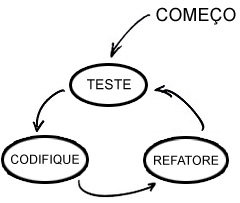
\includegraphics{figuras/tdd}}
    \caption{Fluxograma do ciclo do TDD}
    \label{tdd}
\end{figure}

\citeonline{ASTELS} define o TDD como um estilo de desenvolvimento onde:
\begin{itemize}
    \item{É mantida uma suíte exaustiva de testes;}
    \item{Nenhum código entra em produção a menos que possua testes associados que o valide;}
    \item{Os testes são escritos primeiro;}
    \item{Os testes determinam que código é preciso escrever.}
\end{itemize}

TDD causa grande impacto na qualidade de um software. \citeonline{BECK} nos auxilia no entendimento dessa premissa ao afirmar que:
\begin{itemize}
    \item{Toda vez que alguém toma uma decisão e não a testa, existe uma grande probabilidade de que esta decisão esteja errada;}
    \item{Funcionalidades de software que não podem ser demonstradas através de testes automatizados simplesmente não existem;}
    \item{Testes nos dão à chance de pensar sobre o que é desejado, independente da forma como a solução será implementada.}
\end{itemize}

De forma geral, ao utilizarmos TDD, deve-se escrever um sólido conjunto de testes, denominado suíte de testes, para a verificação do correto funcionamento do sistema. Esta suíte deverá, idealmente, cobrir todo o código do sistema, provendo confiabilidade ao processo de desenvolvimento de software. Vale ressaltar, que TDD não garante a obtenção de níveis aceitáveis em certos aspectos do software final, como usabilidade, desempenho, entre outros. Muito disto, se deve ao fato de TDD não conseguir extinguir riscos relacionados com a falta, ou definição equivocada, de requisitos \cite{RIBEIRO}.

\section{Sistemas de controle de versão}

Uma das ações mais importantes para permitir que diversos desenvolvedores trabalhem juntos em um mesmo projeto é utilizar um Sistema de Controle de Versão (SCV), também conhecido como ``repositório de código'' ou simplesmente ``repositório''. Existem muitos desses sistemas disponíveis no mercado, tais como Subversion, Rational ClearCase, Mercurial, Git, entre outros.

Devido as suas vantagens, os SCVs são sistemas utilizados em muitos tipos de projetos, desde os de pequeno porte aos de grande porte, mostrando a importância desses sistemas. Por isso, atualmente, é difícil encontrar um projeto profissional que não use um Sistema de Controle de Versão, ainda mais com a quantidade de softwares livres que constam nessa área e a imensa qualidade que eles apresentam.

Os Sistemas de Controle de Versão fornecem um local para armazenamento dos arquivos de um projeto e também controlam as versões dos mesmos, possibilitando que desenvolvedores trabalhem no mesmo arquivo ao mesmo tempo \cite{SHORE}. Imagine, por exemplo, que em um projeto haja uma classe Calculadora com capacidade apenas de listar e calcular o valor da soma entre dois números, e que o programador implemente multiplicação e divisão entre dois números. Ao armazenar o código atualizado com as novas funcionalidades, o repositório grava uma nova versão desta classe, ou seja, a classe Calculadora original não é simplesmente substituída por uma nova, ao invés disso, o novo código é anexado ao antigo.

No SCV também é possível guardar versões dos arquivos, possibilitando a recuperação dos mesmos de forma análoga a um botão de ``desfazer''. Quando ocorre algum tipo de erro em um arquivo e este é colocado acidentalmente no repositório, este mecanismo nos permite desfazer as alterações do último \textit{commit} (envio das modificações feitas pelo usuário ao repositório de código), e obter o arquivo antigo \cite{SHORE}. Voltando ao exemplo da classe Calculadora, imagine que a primeira versão funcionasse perfeitamente e, ao ser implementada a multiplicação e divisão entre dois números, algum tipo de erro fosse introduzido por falta de atenção. Suponha ainda que este erro só fosse percebido quando a classe já estivesse em produção. Nesse tipo de situação, a possibilidade de controlar versões com um SCV é muito útil, porque permite a obtenção de uma versão anterior rapidamente (a que funcionava) e colocá-la em produção até que a versão mais recente (com problemas) seja corrigida.

\section{Métodos ágeis}

Cansados de fazer software da mesma maneira, um grupo de desenvolvedores se reuniu para discutir sobre formas de aumentar o desempenho de seus projetos. Desta reunião, alguns valores e princípios foram definidos e, com base neles, foi criado o Manifesto Ágil, que pode ser visto na Figura \ref{manifesto_agil}. ``O Manifesto Ágil, criado em 2001, descreve a essência de um conjunto de abordagens para desenvolvimento de software criadas ao longo da última década'' \cite{IMPROVEIT-MANIFESTO}. Dos valores e princípios do Manifesto Ágil são baseados os métodos ágeis de desenvolvimento de software, que contrastam com a maneira tradicional de se desenvolver.

\begin{figure}[ht]
    \centering
    \scalebox{0.7}{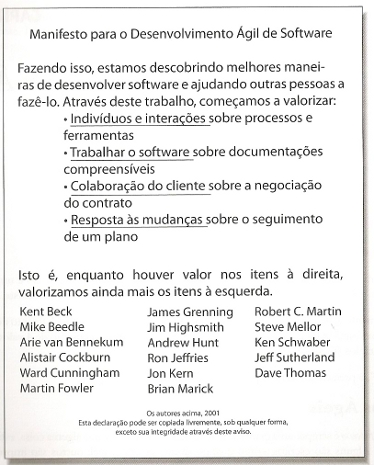
\includegraphics{figuras/manifesto_agil}}
    \caption{Manifesto Ágil. Fonte: \cite{SHORE}}
    \label{manifesto_agil}
\end{figure}

Dos métodos ágeis mais populares, como Scrum, Lean, Crystal, entre outros, uma das metodologias de desenvolvimento que mais se popularizou foi a \textit{Extreme Programming} (XP). Esta, criada por Kent Beck em 1999, é amplamente utilizada em inúmeros projetos ao redor do mundo.

O XP é composto por valores e práticas, e uma destas práticas é a Integração Contínua, tema abordado neste trabalho. A Integração Contínua é uma técnica que foi amplamente difundida com os métodos ágeis \cite{DUVALL-ENTREVISTA}, o que não quer dizer que esta surgiu e somente se encaixa com os métodos ágeis. \citeonline{DUVALL-ENTREVISTA} relata que já trabalhou em projetos que usavam o ciclo de vida ``Cascata'' e, mesmo assim, a equipe utilizava Integração Contínua.

Outros métodos ágeis não possuem como prática a Integração Contínua, porém, são facilmente adaptáveis. O Scrum, por exemplo, não tem a Integração Contínua como prática nativa, mas é perfeitamente adaptável.

\chapter{INTEGRAÇÃO CONTÍNUA}

Neste capítulo é apresentado o referencial teórico sobre a Integração Contínua. São mostrados os tipos de integração, os componentes de um ambiente de Integração Contínua, o \textit{script} que é responsável por integrar o sistema, as práticas e vantagens da Integração Contínua.

\section{O que é Integração Contínua?}
Integração Contínua é um processo que consiste na integração do código fonte pelo menos uma vez ao dia, mantendo a consistência na base de código ao final de cada integração. \citeonline{FOWLER} definiu o processo da seguinte maneira:

\begin{citacao}
Integração Contínua é uma prática de desenvolvimento de software onde os membros de um time integram seu trabalho frequentemente, geralmente cada pessoa integra pelo menos diariamente – podendo haver múltiplas integrações por dia. Cada integração é verificada por um \textit{build} automatizado (incluindo testes) para detectar erros de integração o mais rápido possível. Muitos times acham que essa abordagem leva a uma significante redução nos problemas de integração e permite que um time desenvolva software coeso mais rapidamente.
\end{citacao}

Existem duas formas de executar a integração: a Integração Contínua Síncrona e a Assíncrona.

\subsection{Integração Contínua Síncrona}

Este método de integração, consiste quando o desenvolvedor integra, por vez seu trabalho, compelindo aos outros desenvolvedores esperarem pelo término da integração corrente, para que possam integrar seus respectivos trabalhos \cite{IMPROVEIT-INTEGRACAO}. Por este motivo, nem todos os projetos podem utilizar este método, pois ele exige que os desenvolvedores trabalhem juntos, normalmente em uma mesma sala, garantindo assim, que só um desenvolvedor integre seu trabalho por vez \cite{IMPROVEIT-INTEGRACAO}.

Como o desenvolvedor é obrigado a esperar que seu trabalho seja integrado sem apresentar falhas, isto, certamente, evita que novas tarefas sejam exercidas pelo mesmo, sem que a integração corrente termine. Isto faz com que o desenvolvedor acompanhe detalhadamente todos os testes em tempo de execução, sabendo de imediato se a performance destes está aceitável, consertando-os se necessário. Como consequência disto, nenhum \textit{commit} indevido permanecerá por muito tempo no Sistema de Controle de Versão, visto que o desenvolvedor irá desfazer as alterações que foram enviadas para o repositório caso a integração falhe.

Os componentes deste modelo de integração são representados de acordo com a Figura \ref{componentes_sincrono}.

\begin{figure}[ht]
    \centering
    \scalebox{0.7}{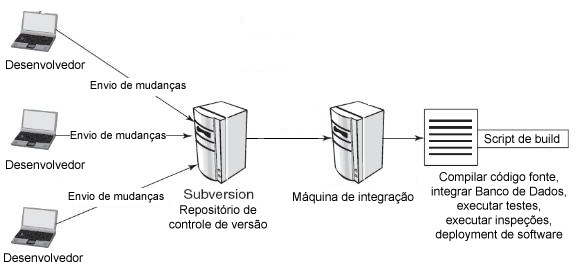
\includegraphics{figuras/componentes_sincrono}}
    \caption{Componentes do modelo de Integração Contínua Síncrona. Adaptado de \cite{DUVALL}}
    \label{componentes_sincrono}
\end{figure}

\subsection{Integração Contínua Assíncrona}

Preferencialmente usada em ambientes em que a equipe está geograficamente distribuída – como em projetos \textit{open source}, por exemplo \cite{IMPROVEIT-INTEGRACAO}. A Integração Contínua Assíncrona consiste basicamente em utilizar um servidor de integração para auxiliar a tarefa de integrar o sistema, ou seja, o processo é feito automaticamente, sem a intervenção direta do desenvolvedor, cujo a única tarefa é submeter as modificações para o SCV, sendo este, monitorado pelo servidor de Integração Contínua, que inicia toda a integração.

Um ponto negativo encontrado nesse modelo de integração refere-se ao fato de uma alteração submetida pelo desenvolvedor que apresentou falhas durante a integração poder criar inconsistência no repositório, uma vez que o responsável por ela pode não estar apto no momento para corrigir tais problemas de forma imediata.

Outro ponto negativo neste modelo trata-se do fato de inúmeras vezes o desenvolvedor só receber a notificação de falha quando já está envolvido em outra tarefa. Isso aumenta o tempo gasto na correção das falhas pelo fato de o desenvolvedor ser compelido a recapitular o contexto mental da tarefa anterior.

Os componentes deste tipo de sistema são representados de acordo com a Figura \ref{componentes}.

\begin{figure}[ht]
    \centering
    \scalebox{0.7}{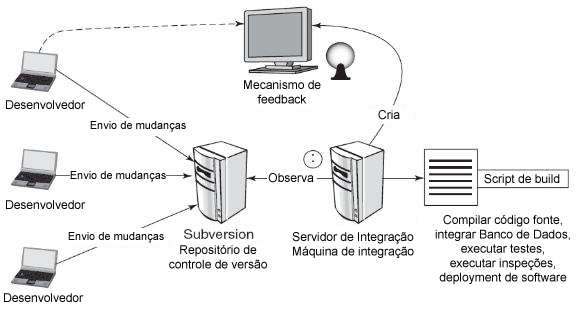
\includegraphics{figuras/componentes}}
    \caption{Componentes de um sistema de Integração Contínua assíncrona. Adaptado de \cite{DUVALL}}
    \label{componentes}
\end{figure}

\section{Componentes de um sistema de Integração Contínua}

Para se obter um sistema de Integração Contínua são necessários vários componentes, em que cada um deles possui sua respectiva responsabilidade. Nas seções seguintes são explicados detalhadamente cada um desses componentes.

\subsection{Desenvolvedor}

O desenvolvedor é a peça fundamental em um sistema de Integração Contínua. Ele é o responsável por realizar as alterações no código fonte do sistema, bem como submeter tais alterações para um Sistema de Controle de Versão, com o intuito de disparar o \textit{script} responsável pela integração do sistema, caracteriznado um cenário de Integração Contínua Assíncrona. De outra forma, o desenvolvedor pode executar este \textit{script} manualmente, caracterizando um cenário de Integração Contínua Síncrona.

\subsection{Sistema de Controle de Versão}

Para um sistema de Integração Contínua, o uso de um Sistema de Controle de Versão é obrigatório, sendo um dos itens mais importantes para todo o processo. O Sistema de Controle de Versão assume tal importância em um sistema de Integração Contínua devido ao fato de que todo o processo é executado através da raiz do repositório. Os SCVs usualmente trabalham com uma \textit{baseline}, ou seja, uma linha principal onde se encontra o código fonte, e é justamente sobre essa linha que todo o processo de integração será executado.

\subsection{Servidor de Integração Contínua}

O servidor de Integração Contínua é o responsável por executar o \textit{script} de integração, também chamado de \textit{build}, quando for encontrada alguma modificação no código fonte que estiver no repositório. Na Integração Contínua Assíncrona, o servidor fica monitorando o repositório do sistema à procura de alterações, coisa que não acontece no modelo de Integração Contínua Síncrona, pelo fato da integração ser feita manualmente.

Essa inspeção que o servidor de Integração Contínua faz, é realizada de tempos em tempos, ou seja, ela ocorre com certa periodicidade. Caso haja alguma modificação no Sistema de Controle de Versão, o servidor irá recuperar os arquivos do repositório e irá rodar o \textit{script} de \textit{build}.

Uma vantagem bastante expressiva nos servidores de Integração Contínua é a capacidade que eles têm de prover uma interface em que os resultados dos \textit{builds} são publicados \cite{FOWLER}. A Figura \ref{buildbot} apresenta o Buildbot\footnote{http://buildbot.net}, um servidor de Integração Contínua, exibindo o resultado da integração de três \textit{builds}, os status destes, as atividades que estão sendo executadas naquele exato momento e as atividades que já foram executadas.

\begin{figure}[ht]
    \centering
    \scalebox{0.7}{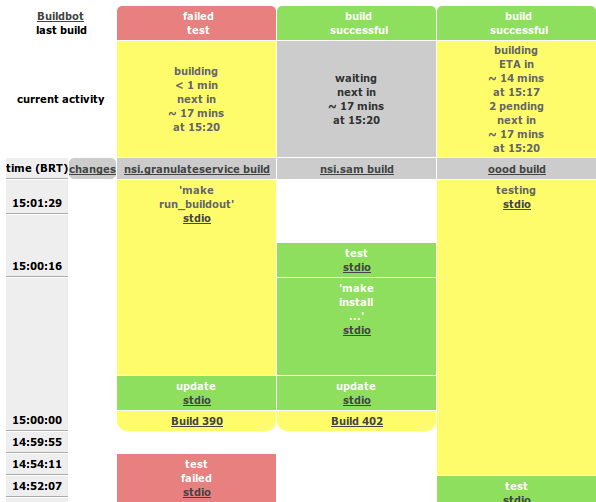
\includegraphics{figuras/buildbot}}
    \caption{Buildbot exibindo dados da integração de um sistema}
    \label{buildbot}
\end{figure}

É recomendável a utilização de um servidor de Integração Contínua quando se deseja automatizar o processo de integração do sistema, porém esta utilização não é obrigatória.

Seguindo a mesma linha dos Sistemas de Controle de Versão, existem muitos servidores de Integração Contínua gratuitos e \textit{open source}, o que viabiliza a implantação de um sistema de integração. Outra recomendação feita é que se tenha uma máquina separada, chamada de máquina de integração, em que todo o processo irá ocorrer. Ela possuirá um servidor de Integração Contínua, que por sua vez irá fiscalizar o Sistema de Controle de Versão em busca de modificações.

\subsection{\textit{Script} de \textit{build}}

``Um \textit{build} é muito mais do que compilar (ou variações das linguagens dinâmicas). Um \textit{build} deve consistir de compilação, testes, inspeção, e \textit{deployment} – entre outras coisas. Um \textit{build} atua como um processo para colocar código fonte junto e verificar se o software trabalha como uma unidade coesiva.'' \cite{DUVALL}.

O \textit{build} é um único \textit{script}, ou conjunto deles, que irá compilar o código fonte do sistema, executar a suíte de testes, realizar a inspeção do código e fazer o \textit{deployment} do software, ou seja, gerar software executável com a última versão do código fonte.

A seção 3.3 - O \textit{script} de \textit{build} apresenta em maiores detalhes as etapas deste \textit{script}.

\subsection{Mecanismo de \textit{Feedback}}

Um dos princípios da Integração Contínua é o \textit{feedback} rápido.Quando uma suíte de teste é executada e caso algum teste falhe, a equipe de desenvolvimento é avisada instantaneamente através do \textit{feedback} \cite{DUVALL}. Recebendo tal informação de falha, o responsável pelo código deve solucionar o problema. O feedback \textit{também} pode ser utilizado para informar a execução do \textit{build} com sucesso, as mudanças no último \textit{build}, os arquivos criados, entre outras coisas.

Em se tratando de Integração Contínua existem várias formas de mecanismo de \textit{feedback}. Pode ser utilizado e-mail, que é a forma mais comum e também o \textit{Short Message Service} (SMS), serviço de envio de mensagens para celulares. Ademais, pode-se obter \textit{feedback} com \textit{Really Simple Syndication (RSS)}, \textit{plugins} de navegadores, mensageiros instantâneos como por exemplo o Google Talk, \textit{widgets}, entre outros.

Além destes mecanismos citados acima, também é comum a utilização de \textit{Ambient Orb} (Orb de Ambiente), que se trata de uma bola que pode ser configurada para ter uma determinada cor específica de acordo com o resultado do \textit{build}. Outro item que também pode ajudar no \textit{feedback} é o som, que pode ser personalizado para executar um determinado arquivo quando o \textit{build} é feito com sucesso. Caso o \textit{build} falhe, o arquivo a ser executado será outro.

Outro mecanismo utilizado são as \textit{Lava Lamps} (Lâmpadas de Lava), as quais são muito conhecidas no mercado como itens decorativos. Elas podem ser configuradas para acenderem de acordo com a situação do \textit{build}. Usualmente formando um par, as lâmpadas costumam ter cada uma delas uma determinada cor. A lâmpada que irá representar o \textit{build} com sucesso terá a cor verde e a lâmpada que demonstrará falha no \textit{build} terá cor vermelha. Enquanto o \textit{build} funcionar, a lâmpada vermelha não irá acender e a verde permanecerá acesa, acontecendo o inverso se o \textit{build} falhar, o que consequentemente irá apagar a lâmpada verde e acender a vermelha. A Figura \ref{lava_lamps} apresenta um exemplo do uso das Lâmpadas de Lava.

\begin{figure}[ht]
    \centering
    \scalebox{0.7}{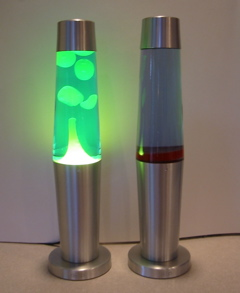
\includegraphics{figuras/lava_lamps}}
    \caption{Lâmpadas de Lava mostrando a situação do \textit{build}. Fonte: \cite{LAVA-LAMPS}}
    \label{lava_lamps}
\end{figure}

Esses mecanismos de \textit{feedback}, como o \textit{Ambient Orb}, as Lâmpadas de Lava e os sons criam um ambiente de trabalho engraçado e personalizado, o que acaba motivando os desenvolvedores e prova que é possível desenvolver software de qualidade em um ambiente descontraído e divertido.

\section{O \textit{script} de \textit{build}}

Essa seção apresenta em detalhes o \textit{script} de \textit{build} bem como seus respectivos tipos e mecanismos.

\subsection{Botão de Integração}

Quando se trata de Integração Contínua, é comum alguns autores citarem o termo ``botão da integração''. O conceito deste, é a criação de um botão virtual, que a um toque, faça com que determinadas etapas sejam executadas e, como resultado final, produzam software funcional. A Figura \ref{botao_integracao} demostra as etapas que são realizadas ao toque do botão da integração.

\begin{figure}[ht]
    \centering
    \scalebox{0.7}{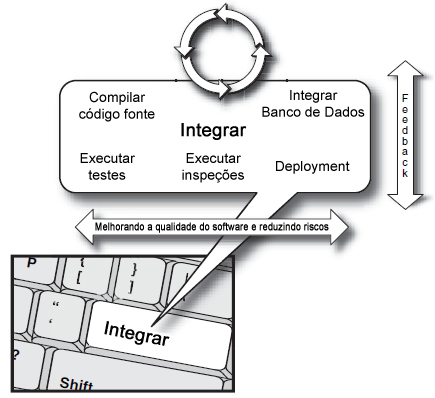
\includegraphics{figuras/botao_integracao}}
    \caption{Botão da integração e suas etapas. Adaptado de \cite{DUVALL}}
    \label{botao_integracao}
\end{figure}

\subsubsection{Compilação de código fonte}

A compilação é uma das etapas mais básicas do \textit{script} de \textit{build}. Compilação se trata do processo de transformação do código fonte em linguagem que a máquina irá entender e executar \cite{DUVALL}.

\subsubsection{Integração de Banco de Dados}

A Integração de Banco de Dados é referente a todo o processamento relacionado ao Banco de Dados do sistema, caso o sistema faça uso de um deles. A Integração do Banco de Dados consiste na execução dos \textit{scripts} de criação e remoção de bancos e tabelas, aplicação de \textit{procedures} e \textit{triggers}, inserção de dados nas tabelas, entre outras coisas.

De acordo com \citeonline{DUVALL}, muitas pessoas acham que a Integração do Banco de Dados é feita como se fosse um processo independente, separado da integração do restante do sistema. Como o Banco de Dados é uma parte que compõe toda a aplicação, o correto é que a cada modificação em um desses \textit{scripts}, o \textit{build} seja executado para verificar se as modificações feitas não geram inconsistência no sistema.

\subsubsection{Execução de testes}

Trata-se de uma das etapas mais importantes do processo de Integração Contínua, uma vez que, ela é responsável pela verificação do correto funcionamento das partes integrantes do sistema, assim como dos relacionamentos entre elas.

\citeonline{FOWLER} apresenta o conceito de \textit{build} auto-testável, onde defende que uma falha ou erro na execução de qualquer um dos testes integrantes da suíte de testes do sistema deve causar a falha de todo o processo de \textit{build}. Essa abordagem, que é permeada de grandes benefícios para o processo de desenvolvimento de software, vem confirmar a indispensabilidade dos testes para o processo de Integração Contínua.

Outra importância acrescentada por \citeonline{DUVALL} à essa etapa é a de conferir confiabilidade ao que está sendo desenvolvido. Segundo ele, sem testes automatizados, é difícil para desenvolvedores ou colaboradores do projeto terem confiança nas mudanças do software.

\subsubsection{Execução de inspeções}

A etapa de execução de inspeções é caracterizada pelo processo de análise do código que foi escrito \cite{DUVALL}. Esta técnica, muita das vezes feita manualmente, é realizada com um  desenvolvedor da equipe criticando e fazendo sugestões ao código que outro desenvolvedor escreveu.

Essa tarefa de inspeção manual de código pode acarretar em desperdício de tempo, visto que seguir padrões são cansativos, dolorosos e difíceis de serem acompanhados.

Para evitar a dor de cabeça causada pela inspeção manual de código, existem ferramentas gratuitas que fazem o processo automaticamente. Elas têm as funcionalidades de verificar código duplicado, quantificar o número de linhas não comentadas e até mesmo fazer um \textit{build} falhar caso algum padrão não tenha sido obedecido.

\subsubsection{\textit{Deployment}}

\textit{Deployment} é o processo que torna possível a entrega do software funcional ao cliente, com as últimas modificações ocorridas, em qualquer lugar, a qualquer hora e com o mínimo de esforço, viabilizando um ambiente de teste para a avaliação do cliente \cite{DUVALL}. Esta entrega é denominada, no método ágil XP, como \textit{release}, e é normalmente feita a pedido do cliente ou negociada no início do desenvolvimento (será entregue ao cliente um software funcional toda semana, por exemplo).

O \textit{deployment} pode ser uma etapa do \textit{script} de \textit{build}, mas normalmente não é, por dois principais motivos: o primeiro, por ser um processo lento que abrange outras etapas, como compilação do código fonte, integração do banco de dados, execução dos testes, execução de inspeções, entre outras coisas; o segundo é pelo fato de que cada \textit{commit} feito para o SCV, faz com que o \textit{script} de \textit{build} seja executado. Visto que, muitos destes \textit{commits} são efetuados por dia,  não entende-se aqui a nescessidade de se ter inúmeras \textit{releases} por dia, já que, elas são a pedido do cliente ou programadas, como já foi mencionado no parágrafo anterior, além de evitar, gastos desnecessários de processamento e de tempo.

\subsubsection{Documentação}

Um dos objetivos do \textit{build} pode ser a criação automática da documentação do software. Para \citeonline{DUVALL}, a melhor documentação acaba sendo o próprio código fonte, quando este apresenta-se de forma clara e concisa atráves de nomes de métodos, variáveis, classes, entre outros. Todavia, somente este código bem escrito, nem sempre é o suficiente. Determinados projetos necessitam de diagramas de UML, documentação de \textit{Application Programming Interface} (API), etc. Gerar esta documentação manualmente é trabalhosa, pois qualquer modificação no código costuma alterar a documentação. Porém, existem ferramentas que criam esta documentação automaticamente, e podem ser embutidas no \textit{script} de \textit{build}, obtendo sempre a documentação atualizada e, consequentemente, evitando desperdício de tempo.

\subsection{Tipos de \textit{build}}

O \textit{build} pode ocorrer em 3 níveis de hierarquia:

\begin{itemize}
    \item{Privado}
    - Neste tipo de \textit{build}, a integração é feita na máquina do desenvolvedor. O desenvolvedor, ou o par (em práticas ágeis), roda um \textit{build} privado antes de enviar o novo código para o repositório, para integrar as mudanças dele com as possíveis mudanças que outros desenvolvedores da equipe tenham feito. As etapas para executar um \textit{build} privado são:
    \begin{enumerate}
        \item{Pegar do repositório o código a ser alterado}
        \item{Fazer as alterações necessárias no código}
        \item{Pegar as últimas mudanças do repositório}
        \item{Rodar o \textit{build} privado}
        \item{Comitar o código modificado para o repositório}
    \end{enumerate}

A Figura \ref{build_privado} apresenta o esquema das etapas para se executar um \textit{build} privado.

\begin{figure}[ht]
    \centering
    \scalebox{0.7}{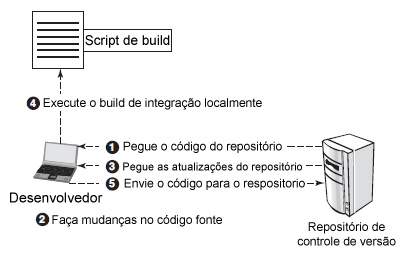
\includegraphics{figuras/build_privado}}
    \caption{Esquema das etapas para se executar um \textit{build} privado. Adaptado de \cite{DUVALL}}
    \label{build_privado}
\end{figure}

    \item{Integração}
    - Este \textit{build} de Integração tem como objetivo integrar todas as mudanças ocorridas no repositório. Ele integra todas as alterações que o desenvolvedor fez, com o código que está localizado no Sistema de Controle de Versão. O ideal é que esse \textit{build} seja executado em uma máquina separada.

    \item{Release}
    - Um dos pilares da Integração Contínua é a possibilidade de se criar software funcionando a qualquer momento com apenas um comando. Este é o objetivo deste \textit{build}, entregar software funcionando para o usuário final, para que ele possa utilizar no ambiente de trabalho dele. Este \textit{build} usualmente é executado com certa periodicidade específica, por exemplo, um mês.
\end{itemize}


\subsection{Mecanismos de \textit{build}}

Nem todos os \textit{builds} são executados da mesma forma. Eles são executados levando-se em consideração o seu propósito e frequência. Alguns \textit{builds} podem ter sua execução feita manualmente por realizar a execução de testes mais demorados, por exemplo. Outros podem ser disparados automaticamente, bastando somente acontecer alguma mudança no Sistema de Controle de Versão. Portanto, existem alguns mecanismos de \textit{build}, como descrito abaixo:

\begin{itemize}
    \item{Sob-demanda} - O processo de \textit{build} é disparado manualmente pelo desenvolvedor.
    \item{Programado} - Neste mecanismo, o \textit{build} é disparado por algum evento pré-definido, como um intervalo de tempo. O \textit{build} será executado independentemente de ter ocorrido, ou não, alguma alteração no repositório de código.
    \item{À procura de mudanças} - Um processo do servidor de Integração Contínua fica sendo executado durante um intervalo de tempo regular em busca de mudanças no repositório do software. Caso haja alguma alteração no código existente, o processo de \textit{build} é disparado automaticamente.
    \item{Guiado por evento} - Mecanismo muito parecido com o de procura por mudanças, porém, o processo de verificação de mudanças no código é feito pelo próprio repositório. Se ele detecta uma mudança, o processo de \textit{build} é inicializado.

A Figura \ref{mecanismos} mostra quais mecanismos cada \textit{build} pode executar.

\begin{figure}[ht]
    \centering
    \scalebox{0.7}{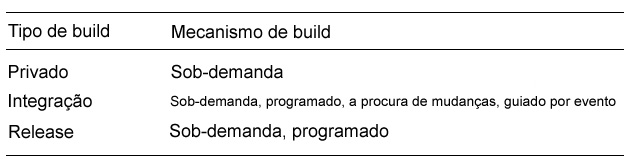
\includegraphics{figuras/mecanismos}}
    \caption{Relação entre mecanismos e tipos de \textit{build}. Fonte: \cite{DUVALL}}
    \label{mecanismos}
\end{figure}
\end{itemize}

\section{Práticas da Integração Contínua}

Neste item é explicado algumas práticas comuns da Integração Contínua.

\subsection{Manter um único repositório de código}

Projetos de software, usualmente, são compostos por várias pessoas. Cada pessoa da equipe irá criar inúmeros arquivos que, em conjunto, resultarão no produto final. Ao longo do projeto, a quantidade de arquivos criados irá crescer rapidamente, o que torna penosa a tarefa de coordenar manualmente todo o trabalho de uma equipe. Para tal serviço é que são utilizados os Sistemas de Controle de Versão, os quais também são chamados de repositórios.

Em um ambiente de Integração Contínua é muito importante a utilização de um Sistema de Controle de Versão, com o intuito de manter todos os arquivos necessários juntos para a construção do sistema. Um problema que acontece muitas vezes nas equipes é que elas não colocam todos os arquivos no repositório, pensando que somente devem estar lá arquivos de código fonte. Logo, vê-se a importância de um sistema para centralização dos arquivos necessários para o sistema.

\subsection{\textit{Build} automatizado}

Gerar software funcional com o código que está no repositório requer a realização de várias etapas como a compilação de código fonte, execução de \textit{scripts}, criação do banco de dados, entre outras. Realizar estas etapas manualmente pode se tornar uma tarefa entediante e inconveniente, visto que estas podem, e devem, ser automatizadas. O patamar ideal é que o software possa ser criado com apenas um simples comando, através de um \textit{script} de \textit{build} automatizado.

Quando é dito que um comando deve criar software funcional, deve-se levar em conta, que todos os arquivos necessários para criar o sistema estejam no \textit{script} de \textit{build}. Então, qualquer pessoa deve ser capaz de pegar uma máquina virgem, obter os arquivos do repositório, executar um único comando e ter um sistema rodando na máquina \cite{FOWLER}. O que acontece muitas vezes é que as equipes esquecem de colocar tudo que é essencial no \textit{build}, fazendo com que, para criar o software final, seja preciso realizar determinadas tarefas, antes ou depois da execução do \textit{script} de \textit{build}.

\citeonline{FOWLER} também diz que o build só deve compilar os arquivos que foram modificados. Com isso, o tempo de execução de um \textit{build} pode ser reduzido consideravelmente, o que é uma prática aconselhável.

Quando se diz em \textit{script} de \textit{build}, imagina-se que ele é apenas um único \textit{script} que faz todo o serviço, e nem sempre é isso, ele também pode ser um conjunto de \textit{scripts}, onde cada um faz uma determinada tarefa. Alguns projetos, por exemplo, possuem testes que são mais demorados, como por exemplo, testes de carga e performance. Esperar por testes demorados em um \textit{build}, obviamente, não é uma boa prática, o que condiz com a prática do XP ``\textit{Ten minute build}'' (Build de dez minutos) \cite{BECK}. Por tal motivo, nem sempre é aconselhável que esses testes fiquem no \textit{script} de \textit{build}. Por isso, é normal que diferentes tipos de \textit{build} sejam criados e que cada um deles execute diferentes tarefas, sendo cada um executado em determinados momentos do projeto.

\subsection{\textit{Build} auto-testável}

Uma boa forma de capturar defeitos mais rapidamente e eficientemente é incluir testes automatizados no processo de \textit{build} \cite{FOWLER}. Levando-se em consideração que um dos princípios da Integração Contínua é o \textit{feedback} instantâneo, uma suíte de testes abrangente é a melhor forma de verificar se o sistema está integrado corretamente.

Com o avanço do método ágil \textit{Extreme Programming} (XP) e a prática \textit{Test Driven Development} (TDD), o desenvolvimento de testes ficou muito mais viável e popular. Apesar destas práticas serem recomendadas, elas não são obrigatórias, pois o que realmente importa para realizar a Integração Contínua é o código coberto por testes, independente da técnica com que eles foram construídos.

Segundo \citeonline{FOWLER}, para que um \textit{build} seja auto-testável, a falha de um teste deve causar a falha do \textit{build}. Daí surge a importância do \textit{build} auto-testável ter uma boa cobertura de testes.

\subsection{Todos enviam alterações para o repositório todos os dias}

De acordo com a definição de \citeonline{FOWLER} acerca da Integração Contínua, os desenvolvedores devem enviar código para o repositório, ao menos uma vez por dia, ou seja, quanto mais \textit{commits} forem feitos pelos desenvolvedores, melhor será o processo de integração.

Enviar código frequentemente para o repositório é uma boa prática, porque reduz conflitos entre os códigos. O que costuma acontecer é a nescessidade de mais de um desenvolvedor ter que trabalhar no mesmo arquivo, o que pode gerar conflitos, pois o código pode ser alterado de tal forma que os testes falhem ao serem executados. Embora esses conflitos aconteçam, quanto mais rápido eles forem descobertos, mais rápido eles serão corrigidos. Imagine que o tempo entre o envio de arquivos para o repositório seja curto. Caso haja conflito, haverão poucos lugares para verificar aonde o problema está. Agora imagine que os arquivos sejam enviados para o repositório com pouca frequência. A quantidade de lugares em que o \textit{bug} pode estar escondido aumenta consideravelmente, dificultando sua resolução.

Além disto, envios frequentes ao repositório encorajam aos desenvolvedores a quebrar seus códigos em pequenas partes de poucas horas cada \cite{FOWLER}. Isto, que combina fielmente com o princípio do método XP, \textit{Baby Steps} (Passos de bebê) \cite{IMPROVEIT-PASSOS}, faz com que o código seja feito gradativamente e com segurança, evitando conflitos e criando a sensação de progresso.

\subsection{Todo \textit{commit} deve atualizar a \textit{baseline} na máquina de integração}

Independente do modelo de Integração Contínua que a equipe estiver utilizando, todo \textit{commit} efetuado deve gerar o sistema com as última modificações encontradas na \textit{baseline} (local do repositório que contém as últimas alterações do sistema), em uma máquina dedicada, a qual é chamada de máquina de integração.

Quando o desenvolvedor altera o código em que está trabalhando, a intenção é que as modificações, que funcionaram em uma máquina, funcionem também nas máquinas dos demais desenvolvedores do projeto \cite{SHORE}. Por este motivo, \citeonline{DUVALL} salienta que o ambiente de trabalho seja exatamente igual ao ambiente de produção. Todavia, nem sempre é isso o que acontece. Muitas vezes, o código que funciona na máquina do desenvolvedor não funciona em outros ambientes. É daí que surge a idéia da máquina de integração. Esta contém um ambiente bom e puro que serve para ratificar que as alterações feitas irão funcionar em qualquer máquina do ambiente de desenvolvimento.

Uma recomendação feita acerca do uso da máquina de integração é que esta só deve ser utilizada para integrar o sistema e não ser usada para correção de problemas \cite{SHORE}. A correção deve ser feita na máquina do desenvolvedor pois, provavelmente, ele deve ter esquecido de realizar o \textit{commit} de um ou mais arquivos. Se o problema for corrigido na máquina de integração, os desenvolvedores que pegarem o código do repositório também irão encontrar os mesmos problemas.

\subsection{Mantenha o {build} rápido}

Segundo \citeonline{SHORE}, o problema mais comum que as equipes que praticam a Integração Contínua enfrentam, são os \textit{builds} lentos e para \citeonline{FOWLER}, o principal foco da Integração Contínua é prover \textit{feedback} rápido. Logo, é impossível obter \textit{feeedback} instantâneo com \textit{builds} demorados. Por isso, existe a recomendação de sempre se manter o \textit{build} rápido.

\citeonline{SHORE} também diz que, sempre que possível, manter o tempo do \textit{build} abaixo de 10 minutos. Aconselha-se este período de tempo, pois é um intervalo em que os desenvolvedores podem conversar entre si sobre o projeto, planejar as próximas tarefas a serem feitas ou, até mesmo, aproveitar o tempo para descansar. Ademais, quanto mais rápido o \textit{build} for, maior o tempo que os desenvolvedores passarão implementando o sistema.

O que faz com que muitos \textit{builds} fiquem lentos, na maioria dos casos, é a execução de testes demasiadamente demorados. As vezes, o mais aconselhável é a criação de outros \textit{scripts} que possam executar esses testes mais demorados separadamente \cite{SHORE}. Por exemplo, testes de carga, desempenho, estabilidade, são testes lentos e não precisam ser executados em cada integração. Separar os testes demorados do restante do \textit{build}, irá reduzir drasticamente o tempo gasto na integração, fazendo com que seja possível atingir o limiar de 10 minutos do \textit{build} \cite{BECK}.

\subsection{Teste em uma cópia do ambiente de produção}

Quando testes são criados, um dos seus propósitos, é evitar que erros apareçam durante a fase de produção do sistema. Por tal motivo, é necessário fazer os testes em uma cópia do ambiente de produção.

Com ambientes de testes e produção diferentes, erros que podem acontecer em um ambiente, podem não acontecer no outro e vice-versa. Esse é o objetivo de testar em abientes parecidos. A chance de um erro imprevisto acontecer em produção é reduzido consideravelmente \cite{FOWLER}.

Idealmente, o ambiente de teste deve ser idêntico ao ambiente de produção, porém, isso nem sempre é possível. Então, o objetivo é chegar o mais próximo possível do clone do ambiente de produção. Para isso, deve-se usar a mesma versão do sistema de banco de dados, sistema operacional, bibliotecas e até mesmo o mesmo IP, \textit{hardware}, etc.

\subsection{Torne fácil para qualquer pessoa o acesso ao último executável}

Segundo \citeonline{FOWLER} uma das partes mais difíceis na construção de um software, é saber se o que está sendo desenvolvido é realmente o que o cliente espera. Conclui-se que para ajudar neste trabalho, o desenvolvedor deve manter um lugar com o executável da última versão do sistema funcionando, para que possa ser demonstradas, testadas ou simplismente vistas pelo cliente as últimas modificações daquela semana \cite{FOWLER}. Vale ressaltar também, que qualquer um pode acessar o referido executável, sem ter a necessidade, de ter acesso ao \textit{build} ou até mesmo possuir algum conhecimento de informática.

\subsection{Todos podem ver o que está acontecendo}

Para \citeonline{FOWLER}, o estado do \textit{build} é uma das coisas mais importantes para comunicação do processo de integração. Dependendo da situação do \textit{build}, a equipe de desenvolvedores sabe quais atitudes deve tomar.

Baseado na informação do \textit{build}, muitos servidores de Integração Contínua possuem uma interface na qual qualquer pessoa pode acessar e ver o andamento do \textit{build}, se ele está em execução, se falhou ou se foi executado sem erros. Já que a situação do \textit{build} está disponível através do servidor, não há necessidade de estar no mesmo local da equipe para ver seu status, ou seja, pessoas dispersas geograficamente do local da equipe poderão acompanhar o \textit{build}. A Figura \ref{hudson} mostra o Hudson\footnote{http://hudson-ci.org}, um servidor de Integração Contínua, mostrando o status dos \textit{builds} de um determinado projeto.

\begin{figure}[ht]
    \centering
    \scalebox{0.7}{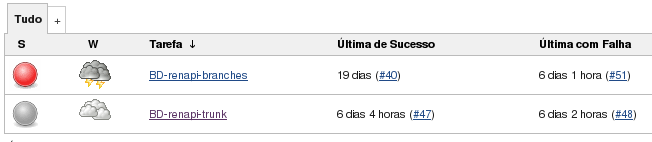
\includegraphics{figuras/hudson}}
    \caption{Status dos \textit{builds} no Hudson.}
    \label{hudson}
\end{figure}

\subsection{\textit{Deploy} automático}

Segundo \citeonline{FOWLER}, é importante ter \textit{scripts} que permitam a implantação da aplicação dentro de qualquer ambiente facilmente. Utilizando \textit{deploy} manual, a implantação do sistema pode não ser aplicada tão facilmente, como disse Fowler. Fazendo uso deste tipo de \textit{deploy}, o responsável deve seguir uma série de etapas para disponibilizar a nova aplicação no ambiente de produção. Exemplificando, o responsável terá que acessar o servidor de produção, parar o servidor \textit{Web}, fazer \textit{backup} da aplicação que está em uso, colocar a nova aplicação e inciar o servidor \textit{Web}. Agora imagine que haja mais etapas a serem realizadas do que as que foram citadas anteriormente. A probabilidade do responsável esquecer alguma etapa aumenta consideravelmente.

Já com o \textit{deploy} automático, a chance de alguém esquecer alguma configuração é extinta, ao passo que no \textit{deploy} manual é necessário realizar várias etapas manualmente. Com a execução de um \textit{script}, as tarefas que eram executadas manualmente, passam a ser automatizadas, reduzindo a chance de erros na hora do \textit{deploy}. Além disso, o processo de \textit{deploy} se torna menos trabalhoso, encorajando os desenvolvedores a fazerem mais \textit{deploys} , mantendo a versão em produção sempre atualizada.

\section{Vantagens da Integração Contínua}

Neste item serão apresentado os principais benefícios que a prática da Integração Contínua pode proporcionar.

\subsection{Defeitos são encontrados e corrigidos o quanto antes}

``Visto que a Integração Contínua integra e roda testes e inspeções diversas vezes ao dia, existe uma grande chance de os defeitos serem descobertos quando eles forem introduzidos'' \cite{DUVALL}.

Exemplificando o que foi dito acima, imagine que um sistema funcione corretamente. Após um determinado \textit{commit}, o sistema não é mais integrado corretamente e o \textit{build}, consequentemente, falha. A partir disso, existe uma grande possibilidade de o código que está quebrando o \textit{build} estar neste último \textit{commit}, visto que, foi a partir dele que o sistema passou a não ser integrado corretamente.

Logo, a quantidade de possíveis lugares onde o defeito pode estar contido é baixa, facilitando a detecção e a resolução do mesmo, contribuindo para a integridade do software criado.

\subsection{Feedback instantâneo}

Segundo \citeonline{FOWLER}, o principal foco da integração contínua é o \textit{feedback} instantâneo. O \textit{script} de \textit{build} será responsável por ativar o único, ou vários, mecanismos de \textit{feedback} para alertar a equipe de desenvolvedores que a última integração que ocorreu apresenta falhas e deve ser corrigida o quanto antes, visando sempre manter a base de código consistente.

O propósito do \textit{feedback} é criar uma notificação que irá estimular uma ação rápida e precisa. Para isso, é necessário enviar a informação correta, para as pessoas corretas, no tempo correto e da forma correta \cite{DUVALL}. A informação correta ideal é a notificação do status do \textit{build}, junto do resultado dos testes, das inspeções e do \textit{deployment}. As pessoas corretas dependerão do tipo de informação enviada, ou seja, o ideal é que cada pessoa da equipe receba somente a informação que lhe seja pertinente, visto que enviar \textit{feedback} para todos no projeto, usualmente, faz com que a equipe passe a ignorar as informações recebidas \cite{DUVALL}. O tempo certo é o menor intervalo possível entre o aparecimento do erro e o \textit{feedback} à equipe. Receber o \textit{feedback} de um \textit{build} quebrado dias atrás não acrescenta em nada à equipe e ainda pode ocasionar perda de tempo e frustração ao alocar desenvolvedores para corrigir um erro que já havia sido corrigido. A forma correta se resume na escolha de um ou mais tipos de mecanismos de \textit{feedback}. O critério de escolha será da própria equipe, levando-se em consideração as vantagens e desvantagens de cada mecanismo.

Com o \textit{feedback} instantâneo, uma modificação que não foi integrada corretamente com o restante do código é rapidamente descoberta, pois o desenvolvedor irá obter uma mensagem caso o \textit{build} tenha quebrado. Corrigir esse erro torna-se muito mais fácil devido à pequena gama de lugares onde o erro pode estar. Agora, imagine que em um sistema a integração seja feita somente após o término do desenvolvimento. Provavelmente, irão surgir erros e mais erros de todos os possíveis lugares, o que torna a correção deles uma tarefa trabalhosa e cansativa.

Além do que já foi dito, o \textit{feedback} irá mostrar o status do sistema. Este mostra para a equipe como está a saúde do software. Verificando a integridade dele é exequível analisar possíveis problemas no processo de integração. Uma base de dados que se mantém por muito tempo corrompida, indica que a equipe não está levando o processo tão sério quanto deveria.

\subsection{Redução de problemas futuros na instalação do software}

Segundo \citeonline{DUVALL}, através da reconstrução e teste de software em um ambiente limpo, ou seja, em um sistema recém-instalado, usando o mesmo processo e \textit{scripts} que foram utilizados no ambiente de desenvolvimento, é possível reduzir problemas futuros na instalação do software. Para exemplificar, supõe-se que uma determinada funcionalidade do sistema tenha como dependência uma pacote chamado ``python-dev'', e que por coincidência, esse pacote já se encontra instalado no ambiente do desenvolvedor. Logo, como o desenvolvedor desconhece desta dependência, ele não o adiciona na lista de dependências do sistema, e sua nova funcionalidade é eviada para o SCV.

Obviamente, quando esta funcionalidade for instalada no servidor de produção, a nova funcionalidade não funcionará. Por este motivo, que deve-se executar os testes, bem como instalar os módulos do sistema em um ambiente recém-instalado, facilitando a detecção deste problema.

\subsection{Redução de processos manuais repetitivos}

É da tendência do ser humano automatizar processos manuais que são feitos com grande frequência. A escassez de tempo e o retrabalho são as principais causas do processo de automatização. Por isso, a existência de máquinas e processos automatizados, já que estes diminuem os custos e aumentam a velocidade da produção \cite{LACOMBE}.

Neste âmbito, a Integração Contínua visa reduzir processos repetitivos economizando tempo, custos e esforço, através da automatização da integração. Estes processos repetitivos podem ocorrer em todas as atividades do projeto, incluindo a compilação do código, integração do banco de dados, testes, inspeções, implantação e \textit{feedback} \cite{DUVALL}.

Para \citeonline{DUVALL}, ao automatizar a Integração Contínua, tem-se uma maior capacidade para assegurar o seguinte:

\begin{itemize}
    \item{O processo funciona da mesma maneira toda vez;}
    \item{Um processo ordenado é seguido. Por exemplo, pode-se executar inspeções (Análise estática) antes de executar os testes - em seu \textit{scripts} de build;}
    \item{A redução do trabalho em processos repetitivos, liberando as pessoas para realizarem trabalhos mais instigantes, de maior valor.}
\end{itemize}

\subsection{Geração de software executável ao clique de um botão}

Quando se fala em geração de software com o clique de um botão, faz-se referência ao botão da integração (Figura \ref{botao_integracao}). A partir deste botão virtual, uma série de etapas é executada, sendo que uma delas é responsável pelo \textit{deployment} do sistema, ou seja, a criação do software executável.

Para \citeonline{DUVALL}, o maior benefício da Integração Contínua é conseguir gerar software executável a qualquer momento, visto que é o item mais ``tangível''  para pessoas que não estão envolvidas diretamente com o desenvolvimento do software, como clientes e usuários.

O fato de o software poder ser gerado a qualquer momento, evita que haja atrasos na entrega do mesmo, para que o cliente possa, por exemplo, testá-lo. Projetos que não usam a Integração Contínua, terão que integrar, rodar inspeções e testes, antes da entrega do sistema. Como a integração manual não é um ``mar de rosas'' e a equipe não integra frequentemente, a quantidade de testes e inspeções que irão falhar será enorme e a integração do sistema não acontecerá corretamente, obrigando a equipe de desenvolvimento a consertar estes defeitos. Em consequência disto, a entrega do software pode atrasar em alguns dias, ou até mesmo meses, devido ao tempo gasto para a correção dos defeitos.

Vale lembrar que ``o objetivo é estar tecnologicamente pronto para o lançamento, mesmo que não esteja funcionalmente pronto para o lançamento'' \cite{SHORE}. Isso mostra que a Integração Contínua pode prover a criação do software a qualquer momento, mesmo que alguma funcionalidade não tenha sido implementada por completo. Suponha que em um sistema, esteja sendo implementado uma nova funcionalidade de cadastro de pessoas. Se em algum momento for necessário a criação do software, ele estará apto para tal, mesmo que não esteja com a funcionalidade totalmente pronta.


\chapter{ESTUDO DE CASO}

Este capítulo apresenta um estudo de caso com a implantação de um ambiente de Integração Contínua no projeto da Biblioteca Digital da Rede Nacional de Pesquisa e Inovação (RENAPI). Este estudo de caso foi idealizado devido ao fato do processo de Integração Contínua realizado no Núcleo de Pesquisa em Sistema de Informação (NSI) do IFF-Campos apresentar problemas, junto com o ideal de melhorar a prática de integração no grupo.

\section{Ambiente estudado}

O estudo de caso deste trabalho foi realizado no NSI. O NSI surgiu em abril de 2002 e desde essa época vem utilizando e estimulando o uso de tecnologias de software livres.

Durante a fase de criação deste estudo de caso, o núcleo contava com 32 bolsistas, subdivididos entre vários projetos. Dois destes projetos estavam diretamente relacionados com este trabalho: o projeto da Biblioteca Digital da RENAPI e o Quali-Ágil.

O portal da Biblioteca Digital da RENAPI visa disponibilizar um acervo bibliográfico digital de maneira a contribuir para a disseminação do material científico e tecnológico produzido na rede de Instituições de Educação Profissional Científica e Tecnológica (EPCT) - como artigos, monografias, dissertações, teses e periódicos, promovendo a disseminação nacional e internacional deste conteúdo, visando colaborar na qualificação do material humano da rede e na disseminação de conhecimento.

O Quali-Ágil é um projeto, que visa o estudo e desenvolvimento de ferramentas e metodologias para aumentar a qualidade de projetos de software que usam metodologias ágeis.

A Biblioteca Digital é um dos projetos mais importantes do NSI. Por tal motivo, ele precisa ser estável e confiável, devido a seu grande porte e visibilidade. Para alcançar tais objetivos, a Integração Contínua é uma boa prática. O papel do Quali-Ágil neste trabalho foi ajudar no gerenciamento e implantação do ambiente de Integração Contínua.

\section{Situação anterior}

O NSI não tinha um processo de Integração Contínua consistente. O processo era feito da seguinte maneira: O Buildbot, servidor de Integrção Contínua utilizado pelo NSI, não tinha o papel característico dos servidores de integração, cuja tarefa é fiscalizar o repositório à procura de mudanças. O Buildbot ficou responsável por executar o \textit{script} de \textit{build} em um determinado horário todos os dias, caracterizando o mecanismo de \textit{build} programado. Da forma como era feita a integração no NSI, o modelo de integração utilizado era o Assíncrono.

O \textit{script} de \textit{build} criado utilizava o Buildout\footnote{http://www.buildout.org/}, sendo esta uma ferramenta \textit{open source} de construção de software criada em Python\footnote{http://www.python.org/}, fornecendo suporte à criação de aplicações.

Quando chegava a hora do \textit{build} ser executado, ele compilava todo o sistema e executava a suíte de testes. Caso algum teste falhasse, a equipe de desenvolvimento recebia um e-mail, sendo este o mecanismo de \textit{feedback} escolhido, com a notificação da falha do \textit{build}.

\section{Problemas}

Uma recomendação para ambientes que usam a Integração Contínua é sempre manter a base de dados estável. Por indisciplina da equipe esta recomendação não era atendida já que, toda vez que algum teste não passava, a equipe recebia a notificação pelo e-mail e mesmo assim o código do repositório ficava inconsistente por muito tempo. A medida correta a ser tomada era corrigir o erro o quanto antes, entretanto o que acontecia era a persistência do erro por dias, ou até mesmo, meses.

Ademais, como a execução do \textit{build} acontecia somente à noite, caso o mesmo viesse a falhar, a tarefa de descobrir a localização do erro era mais difícil. Muitos \textit{commits} eram realizados no período da tarde, todavia nenhum deles ativava o \textit{script} de \textit{build}. Dessa forma, quando o \textit{build} quebrava, era mais difícil saber qual \textit{commit} fez o \textit{build} falhar, visto que foram realizados vários envios de código naquele determinado dia.

O \textit{feedback} da integração não era instantâneo, já que o \textit{build} era programado e só era executado em determinado horário do dia. Logo, para o desenvolvedor saber se a alteração que ele enviou para o repositório foi integrada corretamente, ele precisava esperar até o outro dia para saber o resultado da integração.

Além disso, a idéia do botão da integração não era completa, pois não se conseguia ter software funcional com apenas o clique de um botão. De acordo com o princípio do botão da integração, com apenas um comando deve ser gerado software funcional. Para se obter o software final era necessário a realização de uma série de etapas manuais, o que não condiz com a idéia do botão da integração.

\section{Proposta para implantação da Integração Contínua}

Como a Biblioteca Digital é um projeto de grande porte que está em andamento, decidiu-se por utilizar o modelo de Integração Contínua Assíncrona por este ser de mais rápida implantação e adaptação, comparado com o modelo de integração Síncrono.

O processo começava com os desenvolvedores obtendo o código do repositório da RENAPI para realizar as alterações. Após modificar o código fonte, os desenvolvedores executavam a suíte de testes à procura de falhas. Obviamente, se alguma falha fosse encontrada, eles teriam que corrigí-la. Caso contrário, eles enviariam o código alterado para o repositório da RENAPI.
Nesse estágio, havia uma máquina de integração que possuia um servidor de Integração Contínua, o Hudson. Ele tinha como responsabilidade fiscalizar o repositório da RENAPI constantemente à procura de qualquer modificação no código fonte do projeto. Caso o Hudson encontrasse alguma alteração no repositório, ele iria resgatar e executar o \textit{script} de \textit{build} na máquina de integração. Toda suíte de testes era executada e, se alguma falha acontecesse, o \textit{build} falharia e a equipe de desenvolvimento receberia um e-mail avisando acerca da falha.

O ambiente de Integração Contínua realizado no projeto pode ser visto na Figura \ref{componentes_estudo}

\begin{figure}[ht]
    \centering
    \scalebox{0.7}{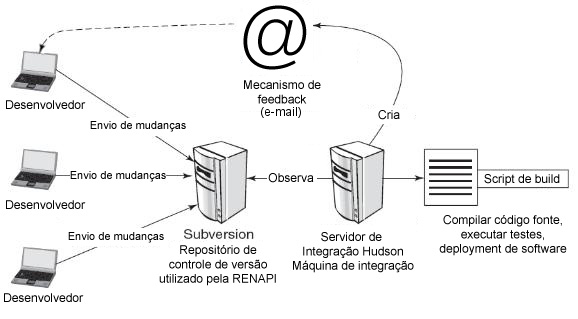
\includegraphics{figuras/componentes_estudo}}
    \caption{Componentes do ambiente de Integração Contínua do estudo de caso.}
    \label{componentes_estudo}
\end{figure}

\section{Como foi feita a implantação}

Para a implantação foi alocada um máquina com processador Pentium 4, 2 GB de Memória RAM e 80 GB de HD. Nesta máquina foi instalado o sistema operacional Debian 5, o mesmo utilizado pelo sistema em produção.

A máquina de integração era totalmente virgem, ou seja, só foi instalado o Debian 5, o Hudson versão 1.357, bem como o Java que é dependência do servidor Hudson. Para instalar o Hudson foi necessário adicionar a chave do repositório Hudson ao sistema com os comandos apresentados na Figura \ref{comandos_chave}.

\begin{figure}[ht]
    \centering
    \scalebox{0.7}{
\includegraphics{figuras/comandos_chave}}
    \caption{Comandos para adicionar chave do repositório Hudson}
    \label{comandos_chave}
\end{figure}

Após isto, bastou somente instalar o Hudson através dos seguintes comandos, como mostra a Figura \ref{comandos_hudson}:

\begin{figure}[ht]
    \centering
    \scalebox{0.7}{
\includegraphics{figuras/comandos_hudson}}
    \caption{Comandos para instalar o Hudson}
    \label{comandos_hudson}
\end{figure}

Instalando o Hudson dessa forma, ele pode ser atualizado pelo gerenciador de pacote do Debian, o apt-get, o que viabiliza o uso da última versão deste servidor de Integração Contínua.

Devidamente instalado, o Hudson foi acessado pela porta 8080, atráves do endereço \textit{http://localhost:8080}. A tela principal do Hudson, pode ser vista na Figura \ref{hudson_principal}

\begin{figure}[ht]
    \centering
    \scalebox{0.6}{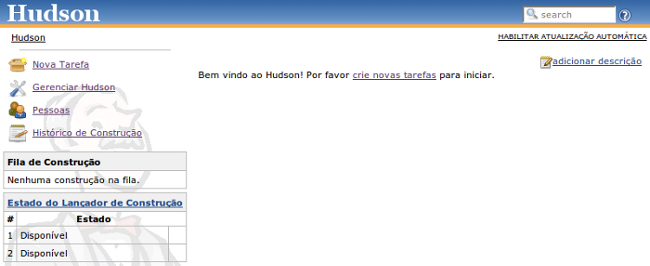
\includegraphics{figuras/hudson_principal}}
    \caption{Tela principal do Hudson}
    \label{hudson_principal}
\end{figure}

O primeiro passo foi fazer a configuração da notificação de e-mail. Caso houvesse alguma falha no \textit{build}, a equipe de desenvolvedores deveria receber um e-mail de notificação da quebra do \textit{build}. Para configurar tal notificação acessou-se o \textit{link} ``Gerenciar Hudson'' na tela principal do Hudson e logo após o ítem ``Configurar Sistema''.

Na seção ``Notificação de E-mail'' o campo ``Servidor SMTP'' foi preenchido com o respectivo servidor de SMTP e o campo ``Endereço de E-mail do Administrador do Sistema'' foi preenchido com o e-mail do responsável pela administração do Hudson. A seção ``Notificação de E-mail'' é demonstrada na Figura \ref{notificacao_email}.

\begin{figure}[ht]
    \centering
    \scalebox{0.7}{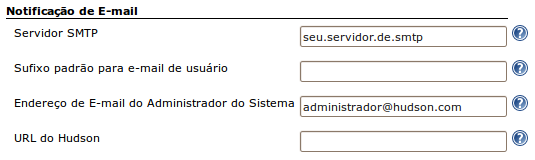
\includegraphics{figuras/notificacao_email}}
    \caption{Tela de configuração da Notificação de E-mail no Hudson}
    \label{notificacao_email}
\end{figure}

Feita a configuração da notificação de e-mail, foi instalado o \textit{plugin} do Selenium\footnote{http://seleniumhq.org/}, que é um \textit{framework} para automatização de testes para aplicações \textit{Web}, sendo este usado nos testes de aceitação do projeto da Biblioteca Digital. Para instalar este \textit{plugin} acessou-se o link ``Gerenciar Hudson'' na tela principal do Hudson e logo após o ítem ``Gerenciar Plugins''. Em seguida foi acessada a aba ``Disponíveis''. Nesta aba, aparecem todos os \textit{plugins} que o Hudson oferece para instalação. Na seção ``Cluster Manegement and Distributed Build (Gerenciamento de \textit{Cluster} e \textit{Build} Distribuído)'' instalou-se o ``Selenium Plugin'', que é responsável por inicializar este \textit{framework}. A instalação do ``Selenium Plugin'' pode ser vista na Figura \ref{selenium_plugin}

\begin{figure}[ht]
    \centering
    \scalebox{0.65}{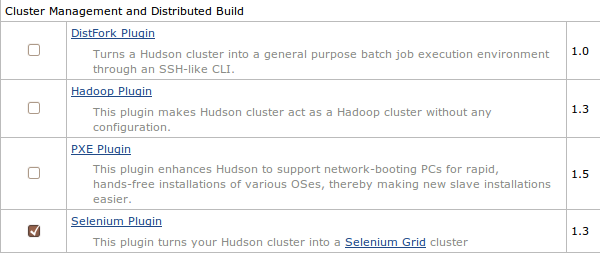
\includegraphics{figuras/selenium_plugin}}
    \caption{Tela de instalação do ``Selenium Plugin'' no Hudson}
    \label{selenium_plugin}
\end{figure}

Após a instalação desse \textit{plugin}, acessou-se no menu lateral esquerdo da tela principal o ítem ``Gerenciar Hudson'', sucedido do ítem ``Manage Nodes (Gerenciamento de Nós)'', que apresenta uma tela de configuração e criação de novos nós. No menu lateral esquerdo, há o ítem ``New Node (Novo Nó)'' que representa a criação de um novo nó. Clicou-se nele e na tela posterior foi preenchido o campo ``Node name (Nome do Nó)'' com o conteúdo ``Selenium Grid'' e selecionado a opção ``Dumb Slave'', como mostra a Figura \ref{hudson_novo_no}.

\begin{figure}[ht]
    \centering
    \scalebox{0.7}{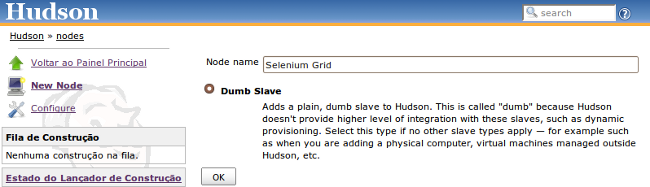
\includegraphics{figuras/hudson_novo_no}}
    \caption{Tela de criação de nós no Hudson}
    \label{hudson_novo_no}
\end{figure}

Na tela seguinte foi nescessário configurar o números de processos concorrentes no processador, para isso foi preenchido o campo ``Número de executores'' com o valor ``10'', ou seja, será permitido 10 processos concorrentes do Selenium no processador. Após isso, o campo ``Diretório de trabalho do sistema remoto'' foi preenchido com o caminho do diretório onde o Hudson deposita seus arquivos de configuração. Em ``Uso'' selecionou-se a opção ``Leave this machine for tied jobs only (Deixar esta máquina somente para trabalhos amarrados)'', o que significa que o nó somente será utilizado quando este for configurado por uma determindada tarefa, permanecendo os demais campos com o valor padrão. Esta configuração pode ser observada na Figura \ref{configuracao_no}.

\begin{figure}[ht]
    \centering
    \scalebox{0.6}{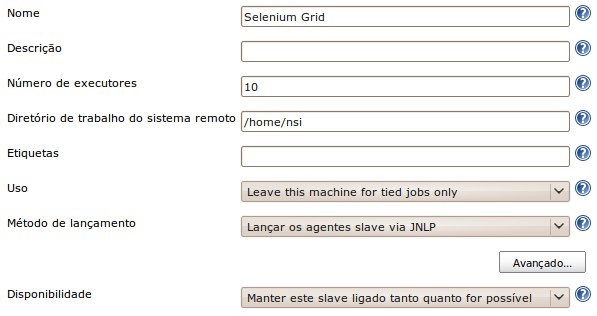
\includegraphics{figuras/configuracao_no}}
    \caption{Tela de configuração de nós no Hudson}
    \label{configuracao_no}
\end{figure}

O próximo passo foi iniciar o nó recém criado, Selenium Grid. Para isso foi pressionado o botão ``Launch (Iniciar)'', e salvo o arquivo ``slave-agent.jnlp'' no mesmo diretório configurado no campo ``Diretório de trabalho do sistema remoto''. Após isso, foi colocado no arquivo /etc/rc.local a linha de comando ``javaws /home/nsi/slave-agent.jnlp'', linha esta que faz com que o Selenium Grid seja inicializado automaticamente, evitando a inicialização manual toda vez que a máquina for ligada.

Depois da configuração do Selenium, acessou-se o link ``Nova Tarefa'' no menu lateral esquerdo da tela principal. Nesta tela, colocou-se o nome da tarefa como ``Biblioteca Digital'' e escolheu-se a opção ``Construir um projeto de software free-style'', como mostra a Figura \ref{hudson_nova_tarefa}.

\begin{figure}[ht]
    \centering
    \scalebox{0.7}{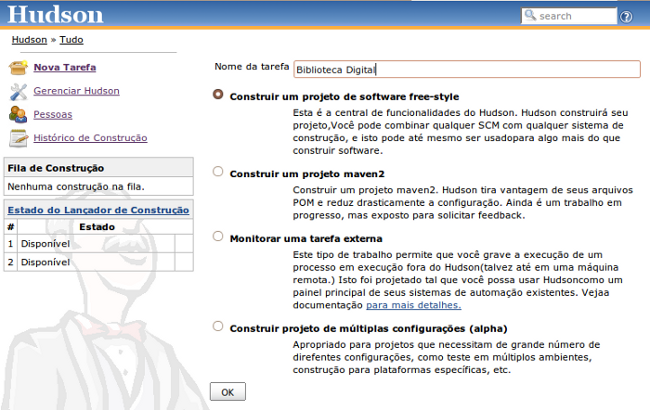
\includegraphics{figuras/hudson_nova_tarefa}}
    \caption{Tela de criação de tarefas no Hudson}
    \label{hudson_nova_tarefa}
\end{figure}

Após preencher os dados requisitados, clicou-se em ``OK'' e uma nova tela foi aberta com dados para configuração da nova tarefa. Na opção ``Tie this project to a node (Amarrar este projeto a um nó)'' escolheu-se o nó criado anteriormente, no caso o Selenium Grid, como demonstra a Figura \ref{configuracao_tarefa_selenium}.

\begin{figure}[ht]
    \centering
    \scalebox{0.7}{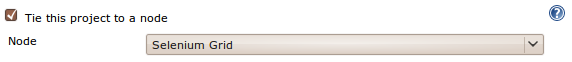
\includegraphics{figuras/configuracao_tarefa_selenium}}
    \caption{Tela de uma tarefa sendo ligada ao Selenium}
    \label{configuracao_tarefa_selenium}
\end{figure}

O próximo passo foi configurar o Sistema de Controle de Versão utilizado pelo projeto da Biblioteca Digital, o Subversion. Na seção ``Gerenciamento de Código Fonte'' foi selecionado a opção ``Subversion'', preencheu-se o campo ``URL do projeto'' com o endereço onde se encontra o repositório da Biblioteca Digital. A opção ``Usar atualização'' foi marcada, para que a cada \textit{build} os arquivos do repostório sejam atualizados automaticamente. A Figura \ref{configuracao_tarefa_subversion} demostra este processo de configuração do Subversion.

\begin{figure}[ht]
    \centering
    \scalebox{0.7}{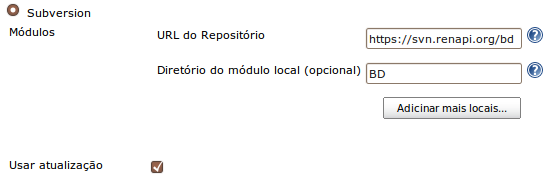
\includegraphics{figuras/configuracao_tarefa_subversion}}
    \caption{Tela de configuração do Subversion em uma tarefa}
    \label{configuracao_tarefa_subversion}
\end{figure}

Na seção ``Disparadores de Construção'' foi marcada a opção ``Consultar periodicamente o SCM''. O campo ``Agenda'' que apareceu, foi preenchido com ``0,30 * * * *'', que segue o padrão Cron, o que significa que o Hudson fiscalizava o repositório no minuto ``0'' e ``30'' de cada hora, todos dias do mês, todos meses e todos dias da semana. Se alguma mudança acontecesse no repositório em alguma dessas fiscalizações, o \textit{build} era disparado. Essa configuração é visualizada na Figura \ref{configuracao_tarefa_consulta}.

\begin{figure}[ht]
    \centering
    \scalebox{0.7}{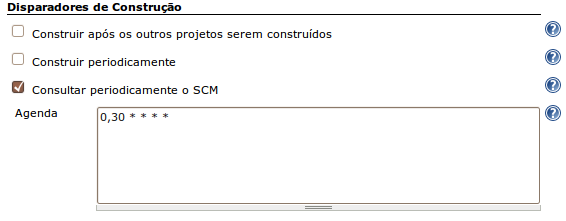
\includegraphics{figuras/configuracao_tarefa_consulta}}
    \caption{Tela de configuração de fiscalização de repositório em um tarefa}
    \label{configuracao_tarefa_consulta}
\end{figure}

Na seção ``Construção'' foi escolhida a opção ``Add Build Step (Adicionar etapa de \textit{build})'' e depois a opção ``Executar shell''. A respectiva caixa da opção ``Executar shell'' foi preenchida com os comandos referentes ao \textit{build}. A Figura \ref{configuracao_tarefa_build} exibe esta etapa.

Por último, na seção ``Ações pós-contrução'', marcou-se a opção ``Notificação de E-mail'' e no campo ``Destinatários'' colocou-se o endereço de e-mail de todos os desenvolvedores da equipe de desenvolvimento da Biblioteca Digital. A Figura \ref{configuracao_tarefa_email} demonstra como fazer esta configuração.

\begin{figure}[ht]
    \centering
    \scalebox{0.7}{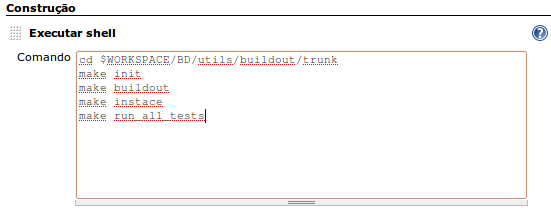
\includegraphics{figuras/configuracao_tarefa_build}}
    \caption{Tela com comandos de execução de um \textit{build} em uma tarefa}
    \label{configuracao_tarefa_build}
\end{figure}

Portanto, esta tarefa foi configurada para obter os arquivos do repositório, executar o \textit{script} de \textit{build}, executar testes e enviar e-mail em caso de quebra do \textit{build}.

\begin{figure}[ht]
    \centering
    \scalebox{0.7}{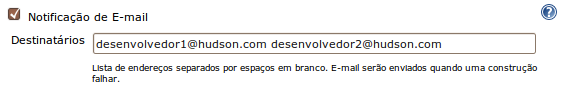
\includegraphics{figuras/configuracao_tarefa_email}}
    \caption{Tela com configuração de envio de e-mail em uma tarefa}
    \label{configuracao_tarefa_email}
\end{figure}

\section{Dificuldades para a implantação}

Uma dificuldade encontrada foi com o \textit{script} de \textit{build}. Para configurar todo o sistema no \textit{script}, foi necessário um esforço maior do que o esperado. O \textit{script} apresentou problemas que exigiram bastante dos desenvolvedores, como por exemplo alguns trechos de código que estavam estáticos, assim dificultando a dinamização do \textit{build}.

Além disso, como o NSI possui muitos desenvolvedores e pesquisadores, alocar a máquina de integração tornou-se uma tarefa difícil. Como a máquina de integração era um computador pessoal (\textit{desktop}), ela ocupava o espaço que um desenvolvedor ocuparia. Aliado a isto, como a máquina deve ser usada exclusivamente para a integração do sistema, nenhuma pessoa deveria fazer uso da máquina.

Outra dificuldade que tomou bastante tempo foi o fato dos testes do projeto estarem falhando. Como o \textit{script} de \textit{build} executava todos os testes do sistema, foram descobertos alguns erros. Logo, como deve-se sempre manter o repositório consistente, alguns dias foram necessários para consertar os erros, inclusive para que o processo começasse de forma correta.

\section{Resultados obtidos}

No estudos de caso desse trabalho foi utilizado um Sistema de Controle de Versão chamado Subversion, que se encontra no endereço https://svn.renapi.org/bd.

O repositório de código era monitorado, e caso alguma mudança fosse detectada, o \textit{script} de \textit{build} era executado, realizando a instalação dos módulos, a execução dos testes, bem como o \textit{deployment} do sistema.

O \textit{build} é auto-testável, ou seja, fazia com que toda a integração do sistema fosse mais facilmente testada.

Uma máquina de integração foi alocada exclusivamente para o processo de integração. Ela não foi utilizada por nenhum desenvolvedor da equipe e continha somente os requisitos necessários para a integração do sistema.

\section{Problemas remanescentes}

A execução dos testes de cada módulo do sistema fez com que testes unitários e de aceitação fossem executados juntos. Com isso, inúmeras inicializações do Selenium eram feitas para execução dos testes de aceitação de cada módulo, acarretando em um tempo maior de \textit{build}. Essas inicializações ocorriam pelo fato do processo do Selenium ser inicializado e finalizado para cada módulo, ou seja, um único processo não poderia ser aproveitado pelos demais módulos. Logo, esse transtorno do Selenium e a alta complexidade do projeto, fizeram com que a integração de apenas cinco módulos estivesse em torno de quarenta minutos.

O sistema inteiro ainda não estava sendo integrado completamente. Somente uma parte do projeto estava inserida no processo de Integração Contínua. Isso ocorria porque integrar todo o sistema iria aumentar exageradamente o tempo de execução do \textit{build}.

O Hudson, que estava sendo executado na máquina de integração, não podia ser visto pelos desenvolvedores da equipe que estivessem fora do IFF. O ideal era que de qualquer lugar, qualquer pessoa pudesse ver como estava a situação do \textit{build} naquele momento.


\chapter{CONCLUSÕES}

\section{Objetivos alcançados}

Com o trabalho realizado foi possível documentar a implantação da Integração Contínua no projeto da Biblioteca Digital da RENAPI.

Com o ambiente de Integração Contínua implantado, mesmo que incompleto, percebeu-se que os desenvolvedores ficam mais confiantes no projeto, visto que a base de código não fica inconsistente por muito tempo. Com toda suíte de testes sendo executada, a confiabilidade do projeto aumenta, bem como a qualidade do código desenvolvido.

Além disso, a documentação criada acerca da teoria da Integração Contínua e da descrição do estudo de caso, criam um bom material para conhecimento da prática e análise de um ambiente de integração em um projeto real.

\section{Trabalhos futuros}

Como o modelo Síncrono de integração é mais confiável e apresenta menos desvantagens do que o modelo Assíncrono, pretende-se utilizar o modelo de Integração Contínua Síncrono ao invés do modelo de Integração Contínua Assíncrono, bastando para isso, disciplinar a equipe para nunca deixar a base de código instável e obter um símbolo de integração para mostrar a equipe quem está integrando naquele exato momento.

Ademais, de acordo com o que foi mencionado na sessaõ 4.8 - Problemas remanescentes, almeja-se separar os testes unitários dos testes de aceitação para agilizar o processo de \textit{build}. Para dinamizar a integração, os testes de aceitação podem ser executados somente uma vez no dia, enquanto os testes unitários devem ser executados a cada \textit{commmit}. Com a redução do tempo do \textit{build}, almeja-se também, fazer a integração de todos os módulos do sistema.

\bibliography{referencia}
%\include{apendice_a}
\end{document}
